\documentclass{beamer}
\usetheme{Warsaw}
\usepackage{nhtvslides}
\usepackage{graphicx}
\usepackage{listings}
\lstset{language=CAML,
basicstyle=\ttfamily\footnotesize,
frame=shadowbox,
breaklines=true}
\usepackage[utf8]{inputenc}

\title{Differential equations}

\author{Dr. Giuseppe Maggiore}

\institute{NHTV University of Applied Sciences \\ 
Breda, Netherlands}

\date{}

\begin{document}
\maketitle

\begin{frame}{Table of contents}
\tableofcontents
\end{frame}

\section{Introduction}
\begin{slide}{Introduction}{Differential equation}{
\item Equations of the form $\dot x = f(x,t)$
\item $x$ is the state of the system (an ``array of floats'')
\item $f$ is the function that computes the derivative of $x$ with respect to time
\item General purpose toolbox for dealing with them
}\end{slide}

\begin{slide}{Introduction}{How does this apply to us?}{
\item $x$ is the state of all our rigid bodies
\item $f$ gives us the derivative of the state: velocity, acceleration, \textit{angular velocity}, torque
}\end{slide}

\begin{frame}{Introduction}
\begin{tabular}{| c | c |}
\hline
$x$ & $f(x)$ \\
\hline
position & velocity \\
velocity/linear momentum & acceleration/force \\
rotation & \textit{angular velocity} ($\omega \star R$) \\
angular velocity/angular momentum & angular acceleration/torque \\
\hline
\end{tabular}
\end{frame}

\section{Numerical solutions}
\begin{slide}{Numerical solutions}{Numerical solutions}{
\item We cannot just compute the state at time $t$
\item There is no closed form for it, unless the problem is really simple \footnote{Yeah, you wish :)}
\item We look for an \textit{approximate} solution
}\end{slide}

\begin{slide}{Numerical solutions}{Field of derivatives}{
\item We know how to compute $f$
\item This means that we can compute the \textit{field of slopes} of $x$
}\end{slide}

\begin{frame}{Slope field}
\center
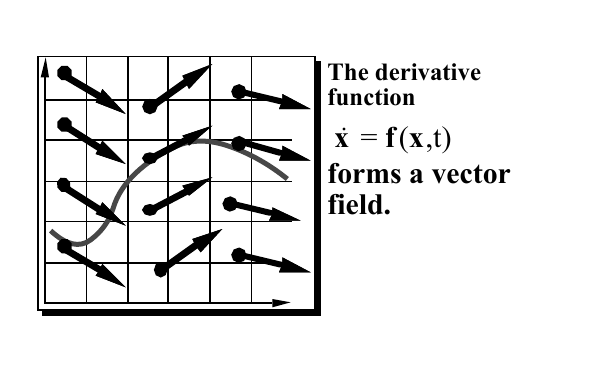
\includegraphics[width=7cm]{Pics/Fig1.png}
\end{frame}

\begin{slide}{Numerical solutions}{Field of derivatives}{
\item Start at $x_0$ 
\item Follow the slope
\item Discrete steps
}\end{slide}

\begin{frame}{Following the slope}
\center
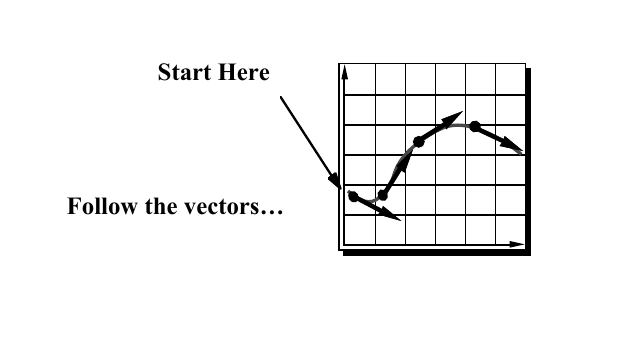
\includegraphics[width=7cm]{Pics/Fig2.png}
\end{frame}

\section{Euler's method}
\begin{slide}{Numerical solutions}{Euler's method}{
\item Big, discrete steps along the slope: $x(t+h) = x(t) + h \dot x(t)$
\item Actually works correctly and \textit{may be acceptable} in some cases
\item If it is acceptable, it's simple to code and fast to run
\item Otherwise it requires a very small time-step to compensate (more computation!)
}\end{slide}

\begin{frame}{Euler's method}
\center
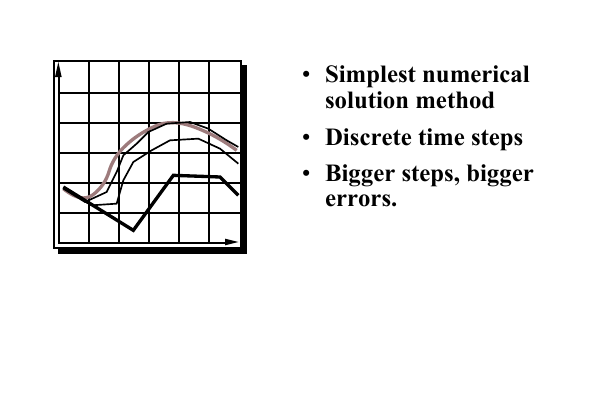
\includegraphics[width=7cm]{Pics/Fig3.png}
\end{frame}

\begin{slide}{Numerical solutions}{Euler's method}{
\item Why may Euler's method not work?
\item Euler's method is
\begin{itemize}
\item Inaccurate, that is it may jump from one trajectory to another
\item Not stable, that is it may increase the energy of the state where it should decrease
\end{itemize}
}\end{slide}

\begin{frame}{Euler's method}
\center
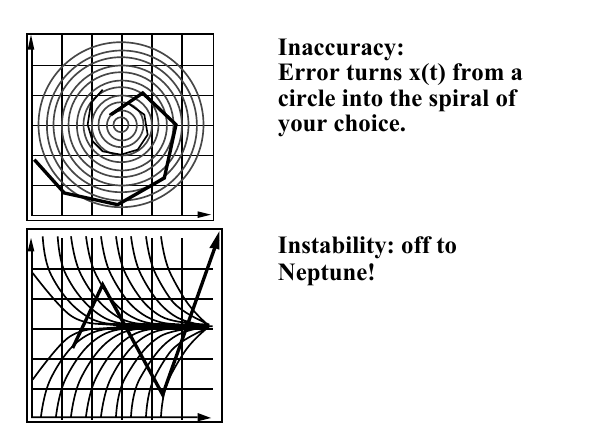
\includegraphics[width=7cm]{Pics/Fig4.png}
\end{frame}

\section{Deriving more sophisticated methods}
\begin{slide}{Numerical solutions}{Taylor series}{
\item Any function can be expressed as the infinite sum of its derivatives
\item $x(t+h) = x(t) + h \dot x(t) + \frac{h^2}{2} \ddot x(t) + \dots + \frac{h^n}{n!} \frac{d^n}{dt^n}x(t) + \dots$
\pause
\item We can \textit{truncate} this summation to \textit{approximate} the original function
\item All differential equations solvers are based on this technique
}\end{slide}

\begin{slide}{Numerical solutions}{Deriving Euler's method}{
\item $x(t+h) = x(t) + h \dot x(t) + \frac{h^2}{2} \ddot x(t) + \dots + \frac{h^n}{n!} \frac{d^n}{dt^n}x(t) + \dots$
\item $x(t+h) \approx x(t) + h \dot x(t)$
}\end{slide}

\begin{slide}{Numerical solutions}{Deriving the midpoint method}{
\item $x(t+h) \approx x(t) + h \dot x(t) + \frac{h^2}{2} \ddot x(t)$
\pause
\item We must now compute $\ddot x(t)$
\item $\ddot x = \frac{d}{dt} \dot x = \frac{d}{dt} f(x(t)) = f'(x(t)) \dot x = f'(x(t)) f(x(t))$
}\end{slide}

\begin{slide}{Numerical solutions}{Deriving the midpoint method}{
\item $\ddot x = f'(x(t)) f(x(t))$
\item We now approximate $f$ with Euler's method
\item $f(x_0 + \Delta x) = f(x_0) + \Delta x f'(x_0)$
}\end{slide}

\begin{slide}{Numerical solutions}{Deriving the midpoint method}{
\item We (arbitrarily) choose $\Delta x = \frac{h}{2} f(x_0)$ (which is an acceptable solution, check units of measure!)
\item Substitute the approximation of $f$
\item $f(x_0 + \frac{h}{2} f(x_0)) = f(x_0) + \frac{h}{2} f(x_0) f'(x_0)$
\item We multiply both sides by $h$:
\item $h(f(x_0 + \frac{h}{2} f(x_0)) - f(x_0)) = \underbrace{\frac{h^2}{2} f(x_0) f'(x_0)}_{\frac{h^2}{2} \ddot x}$
}\end{slide}

\begin{slide}{Numerical solutions}{Deriving the midpoint method}{
\item $x(t+h) \approx x(t) + h \dot x(t) + \frac{h^2}{2} \ddot x(t)$
\item $\ddot x = f'(x(t)) f(x(t))$
\item $h(f(x_0 + \frac{h}{2} f(x_0)) - f(x_0)) = \frac{h^2}{2} f(x_0) f'(x_0) = \frac{h^2}{2} \ddot x$
\pause
\item $x(t+h) \approx x(t) + h \dot x(t) + h(f(x_0 + \frac{h}{2} f(x_0)) - f(x_0))$
}\end{slide}

\begin{slide}{Numerical solutions}{Deriving the midpoint method}{
\item $x(t+h) \approx x(t) + h \dot x(t) + h(f(x_0 + \frac{h}{2} f(x_0)) - f(x_0))$
\item We sample the derivative at the midpoint of the step, hence the name
}\end{slide}

\begin{frame}{RK2}
\center
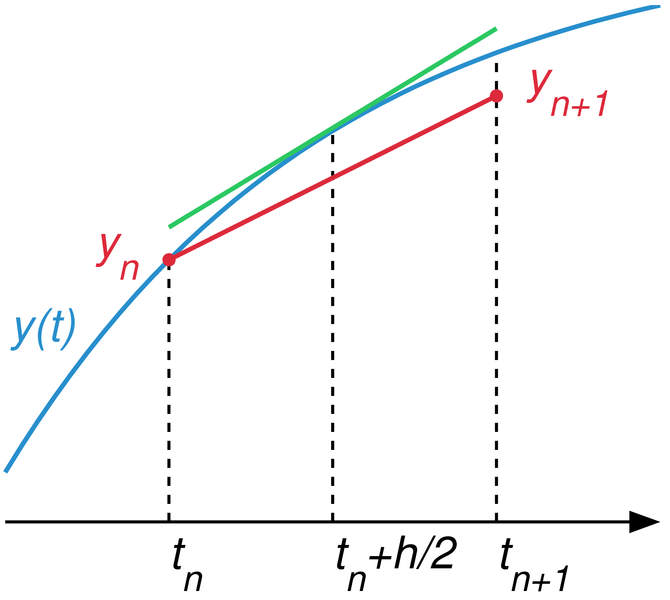
\includegraphics[width=6cm]{Pics/Midpoint_method.png}
\end{frame}

\begin{slide}{Numerical solutions}{About the midpoint method}{
\item $x(t+h) \approx x(t) + h \dot x(t) + h(f(x_0 + \frac{h}{2} f(x_0)) - f(x_0))$
\item We compute $f$ twice; in general though, the higher number of evaluations of $f$ in advanced methods is more than offset by the far smaller time step needed
}\end{slide}

\begin{slide}{Numerical solutions}{RK4}{
\item The ``best'' numerical method though is RK4
\item $k_1 = h f(x_0)$, $k_2 = h f(x_0 + \frac{k_1}{2})$, $k_3 = h f(x_0 + \frac{k_2}{2})$, $k_4 = h f(x_0 + \frac{k_3}{2})$
\item $x(t+h) = x_0 + \frac{1}{6} k_1 + \frac{1}{3} k_2 + \frac{1}{3} k_3 + \frac{1}{6} k_4$
}\end{slide}

\begin{frame}{RK4}
\center
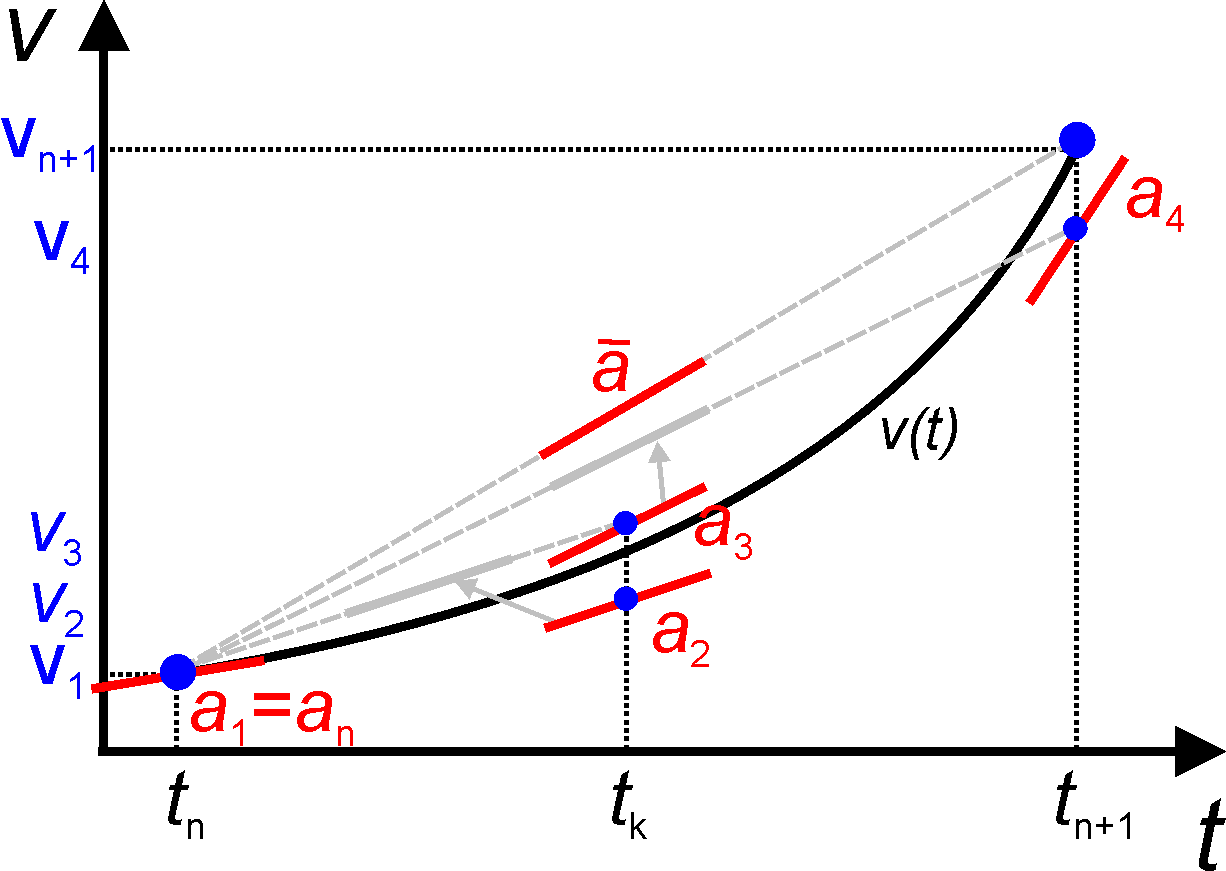
\includegraphics[width=6cm]{Pics/RK4.png}
\end{frame}

\section{The ``best'' method?}
\begin{slide}{Numerical solutions}{To the stars and beyond?}{
\item Why not use RK5, RK6, or even more?
\item Is it not more precise after all?
\pause
\item Suspense :)
\pause
\item NO!
\item We can approximate the higher order derivatives with the first derivative only so far
\item After a while we are just not inserting any new information
\item Very high order methods would only work if we could reliably compute third or fourth order derivatives
\item Otherwise we insert spurious oscillations and new errors in the system
}\end{slide}

\begin{frame}{That's it}
\center
\fontsize{18pt}{7.2}\selectfont
Thank you!
\end{frame}

\end{document}


\begin{slide}{SECTION}{SLIDE}{
\item i
}\end{slide}

\begin{frame}[fragile]{SLIDE}
\begin{lstlisting}
CODE
\end{lstlisting}
\end{frame}

\begin{frame}{SLIDE}
\center
%\includegraphics[height=5cm]{Pics/recursive_multiplier.png}
\end{frame}
